% -----------------------------------------------------------------------------
% Master thesis in the study program computational mechanics
%
% B.Sc. Rezha Adrian Tanuharja - 03751261
% M.Sc. Felix Schneider (supervisor)
%
% chapters/discussion/surrogate/point_B.tex
% Last edited 03 November 2023
% -----------------------------------------------------------------------------

\subsection{Vertical Acceleration at Node B}
\label{ssec: surrogate point B}

Figure \ref{FRF_rRPCE_B_A_16} shows the medians and interquartile ranges of relative empirical errors of the FRF approximations for regular RPCE models at $\omega=16.0$ rad/s.
The medians decrease as the size of the training data increases and converge when the size of the training data is approximately $2.0$ to $2.5$ times the total number of bases in the models.
\begin{figure}[H]
    \centering
    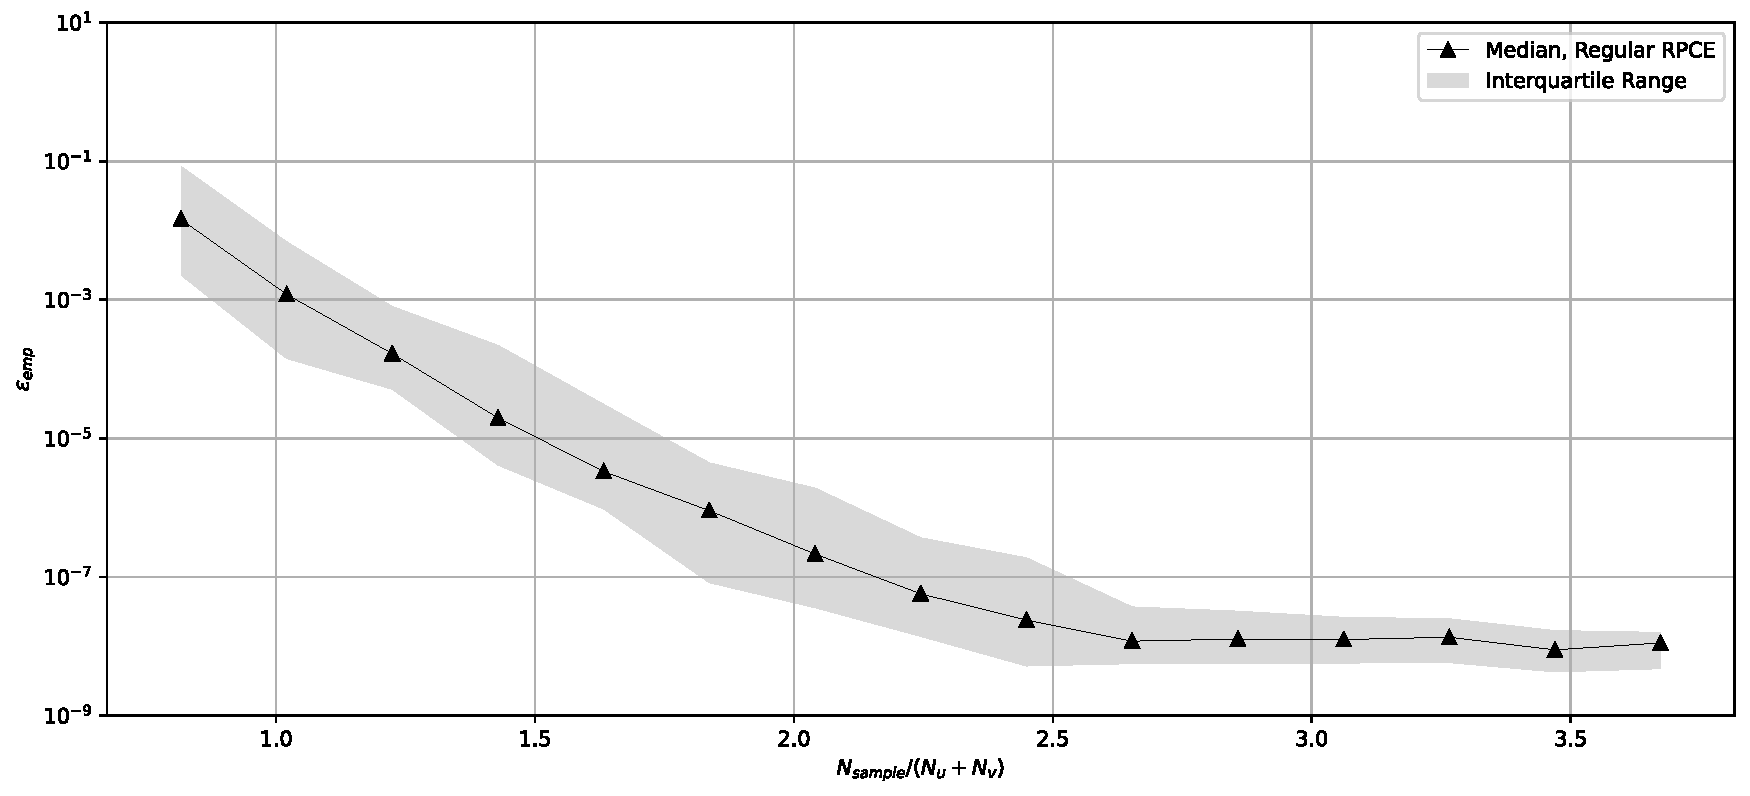
\includegraphics[width=1.0\textwidth]{
        plots/surrogate/plot_1P_B_16.pdf
    }
    \caption{%
        Relative Empirical Errors of $H_{BA}$ for Regular RPCE Models at $\omega=16.0$ rad/s
    }
    \label{FRF_rRPCE_B_A_16}
\end{figure}

Figure \ref{FRF_sRPCE_B_A_16} shows the medians and the interquartile ranges of relative empirical errors of the FRF approximations for regular and sparse RPCE models at $\omega=16.0$ rad/s.
\begin{figure}[H]
    \centering
    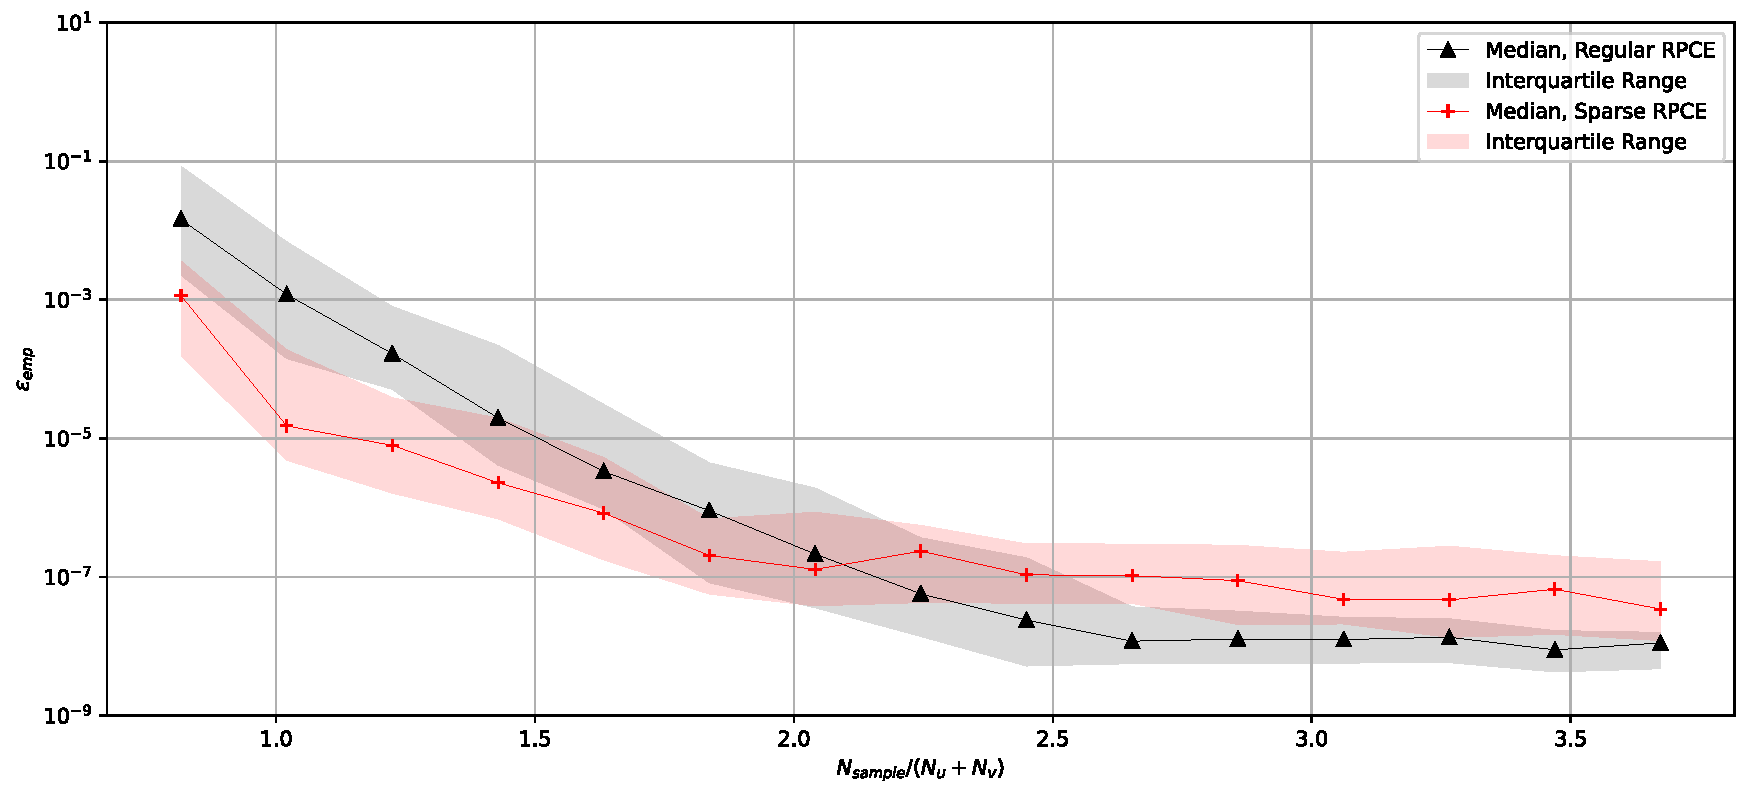
\includegraphics[width=1.0\textwidth]{
        plots/surrogate/plot_1_B_16.pdf
    }
    \caption{%
        Relative Empirical Errors of $H_{BA}$ for Regular and Sparse RPCE Models at $\omega=16.0$ rad/s
    }
    \label{FRF_sRPCE_B_A_16}
\end{figure}
The figure above shows that the sparse RPCE models have lower relative empirical errors when training data sizes are small.
Figures \ref{FRF_sRPCE_B_A_17} to \ref{FRF_sRPCE_B_A_19} show the relative empirical errors of the FRF approximations for regular and sparse RPCE models at various frequencies.
\begin{figure}[H]
    \centering
    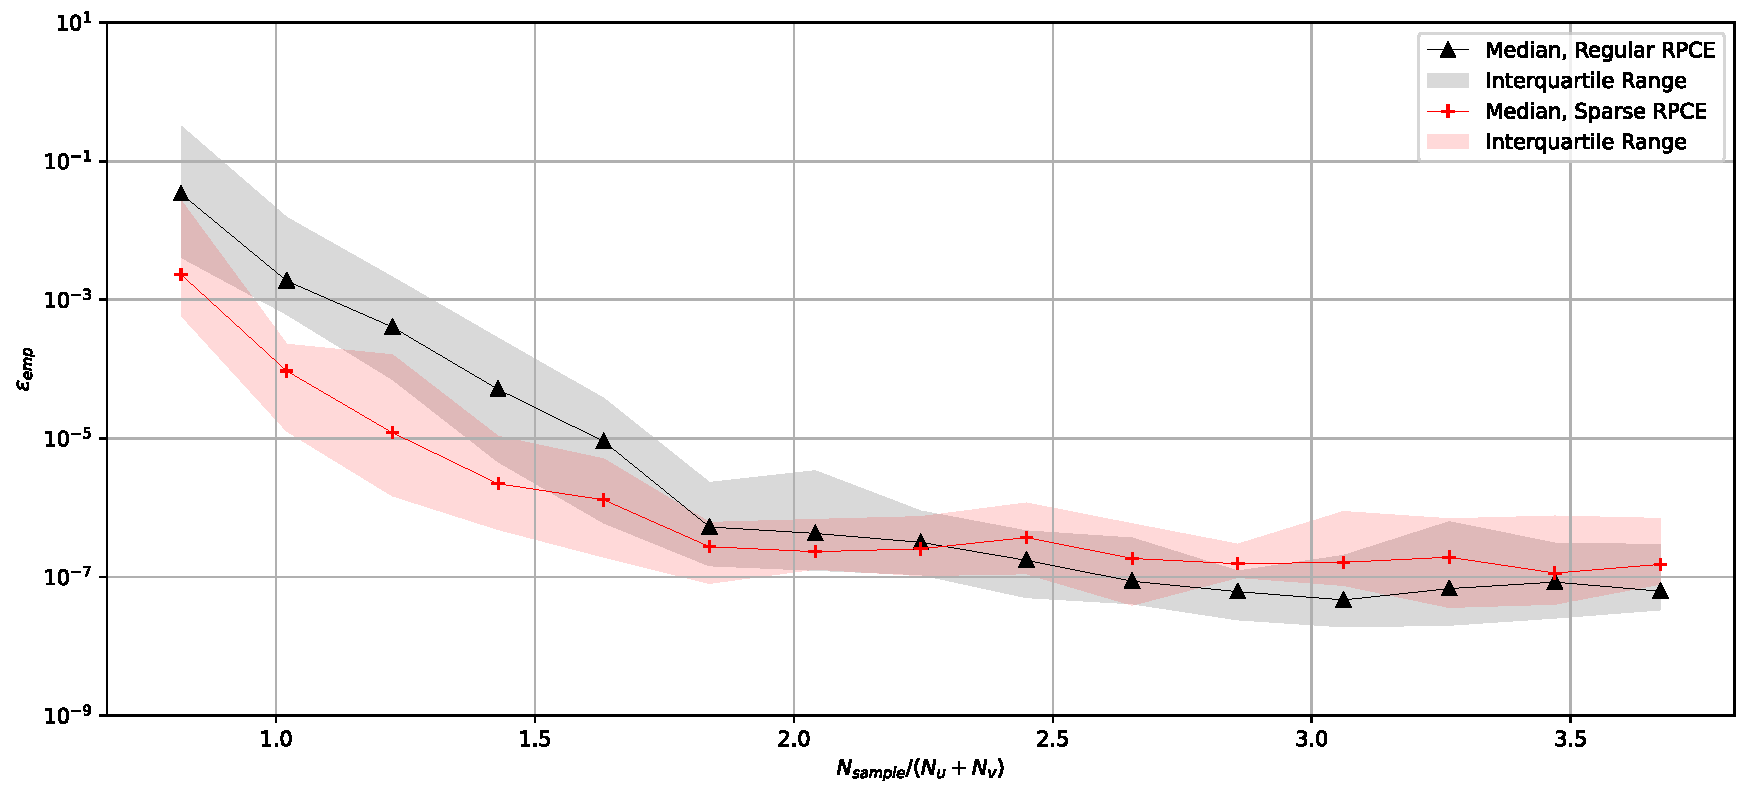
\includegraphics[width=1.0\textwidth]{
        plots/surrogate/plot_1_B_17.pdf
    }
    \caption{%
        Relative Empirical Errors of $H_{BA}$ for Regular and Sparse RPCE Models at $\omega=16.5$ rad/s
    }
    \label{FRF_sRPCE_B_A_17}
\end{figure}
\begin{figure}[H]
    \centering
    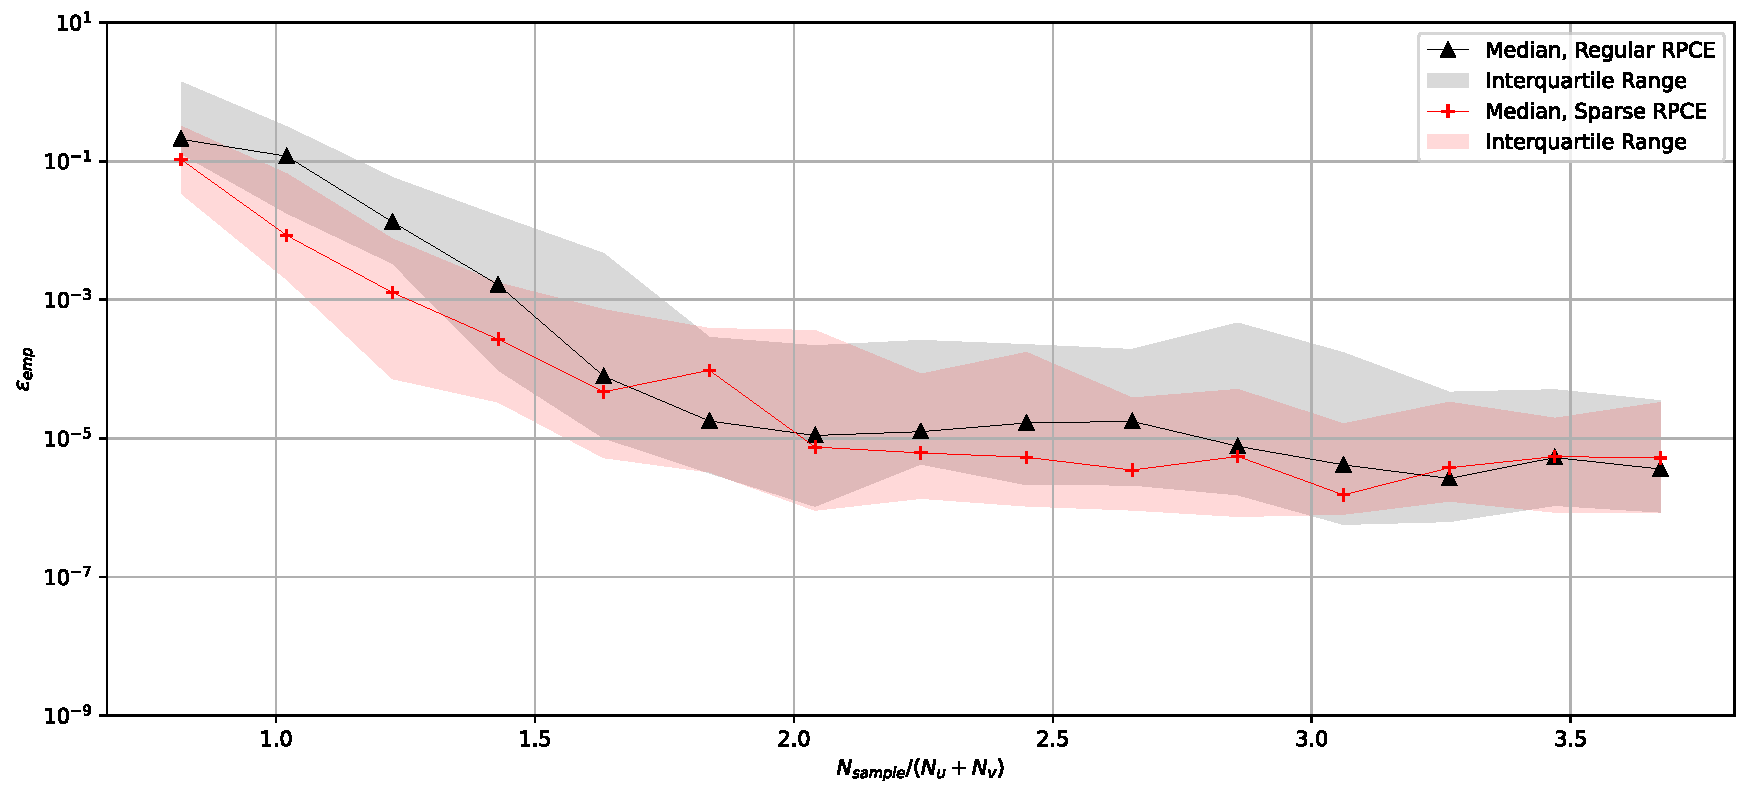
\includegraphics[width=1.0\textwidth]{
        plots/surrogate/plot_1_B_18.pdf
    }
    \caption{%
        Relative Empirical Errors of $H_{BA}$ for Regular and Sparse RPCE Models at $\omega=17.0$ rad/s
    }
    \label{FRF_sRPCE_B_A_18}
\end{figure}
\begin{figure}[H]
    \centering
    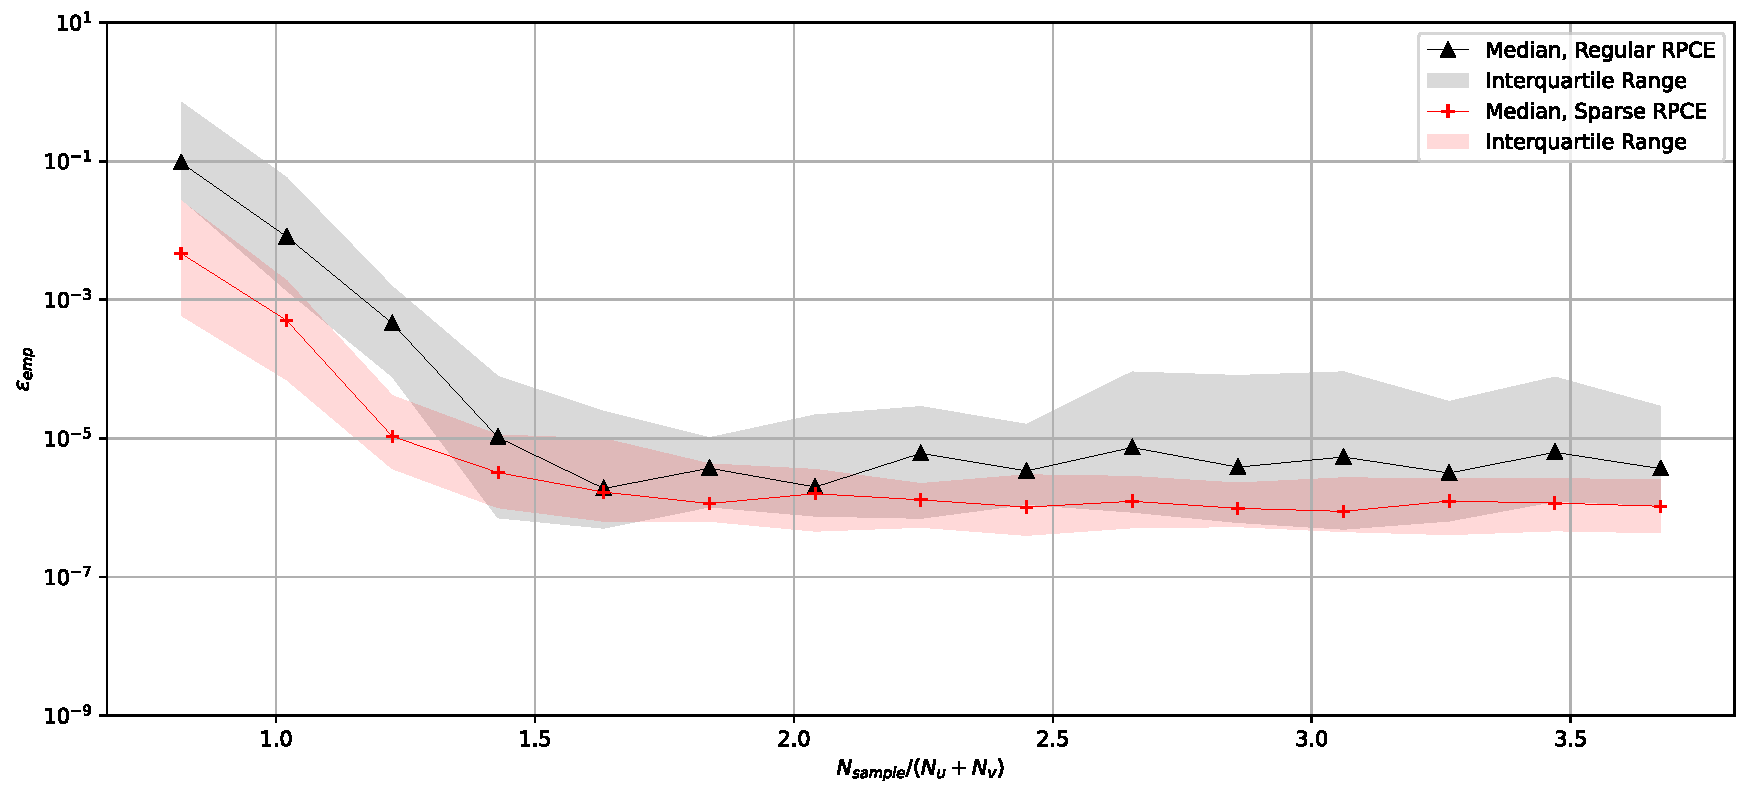
\includegraphics[width=1.0\textwidth]{
        plots/surrogate/plot_1_B_19.pdf
    }
    \caption{%
        Relative Empirical Errors of $H_{BA}$ for Regular and Sparse RPCE Models at $\omega=17.5$ rad/s
    }
    \label{FRF_sRPCE_B_A_19}
\end{figure}
The figures above exhibit the same trends: the sparse RPCE models have lower relative empirical errors when training data sizes are small.
% The relative empirical errors for regular and sparse RPCE models at other frequencies are available in the appendix.

To dive deeper into the difference between the regular and sparse RPCE models, the author evaluates the relative mean and variance error of the approximations.
Figures \ref{mean_rRPCE_B_A_16} and \ref{var_rRPCE_B_A_16} show the relative mean errors and relative variance errors of the FRF approximations for regular RPCE models at $\omega=16.0$ rad/s.
\begin{figure}[H]
    \centering
    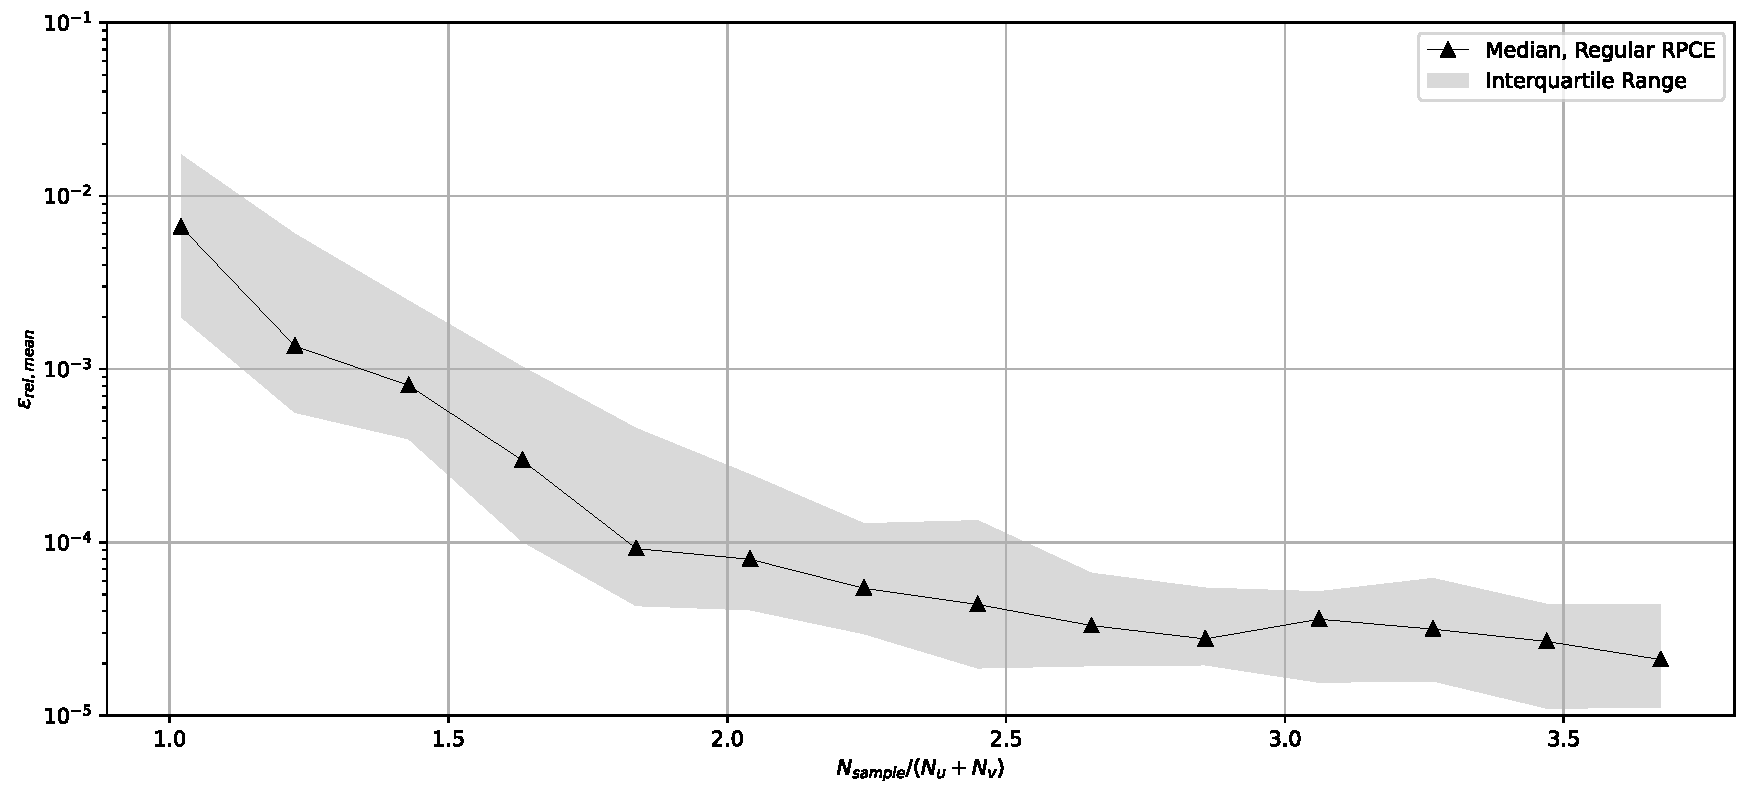
\includegraphics[width=1.0\textwidth]{
        plots/surrogate/plot_2P_B_16.pdf
    }
    \caption{%
        Relative Mean Errors of $\left|H_{BA}\right|$ for Regular RPCE Models at $\omega=16.0$ rad/s
    }
    \label{mean_rRPCE_B_A_16}
\end{figure}
\begin{figure}[H]
    \centering
    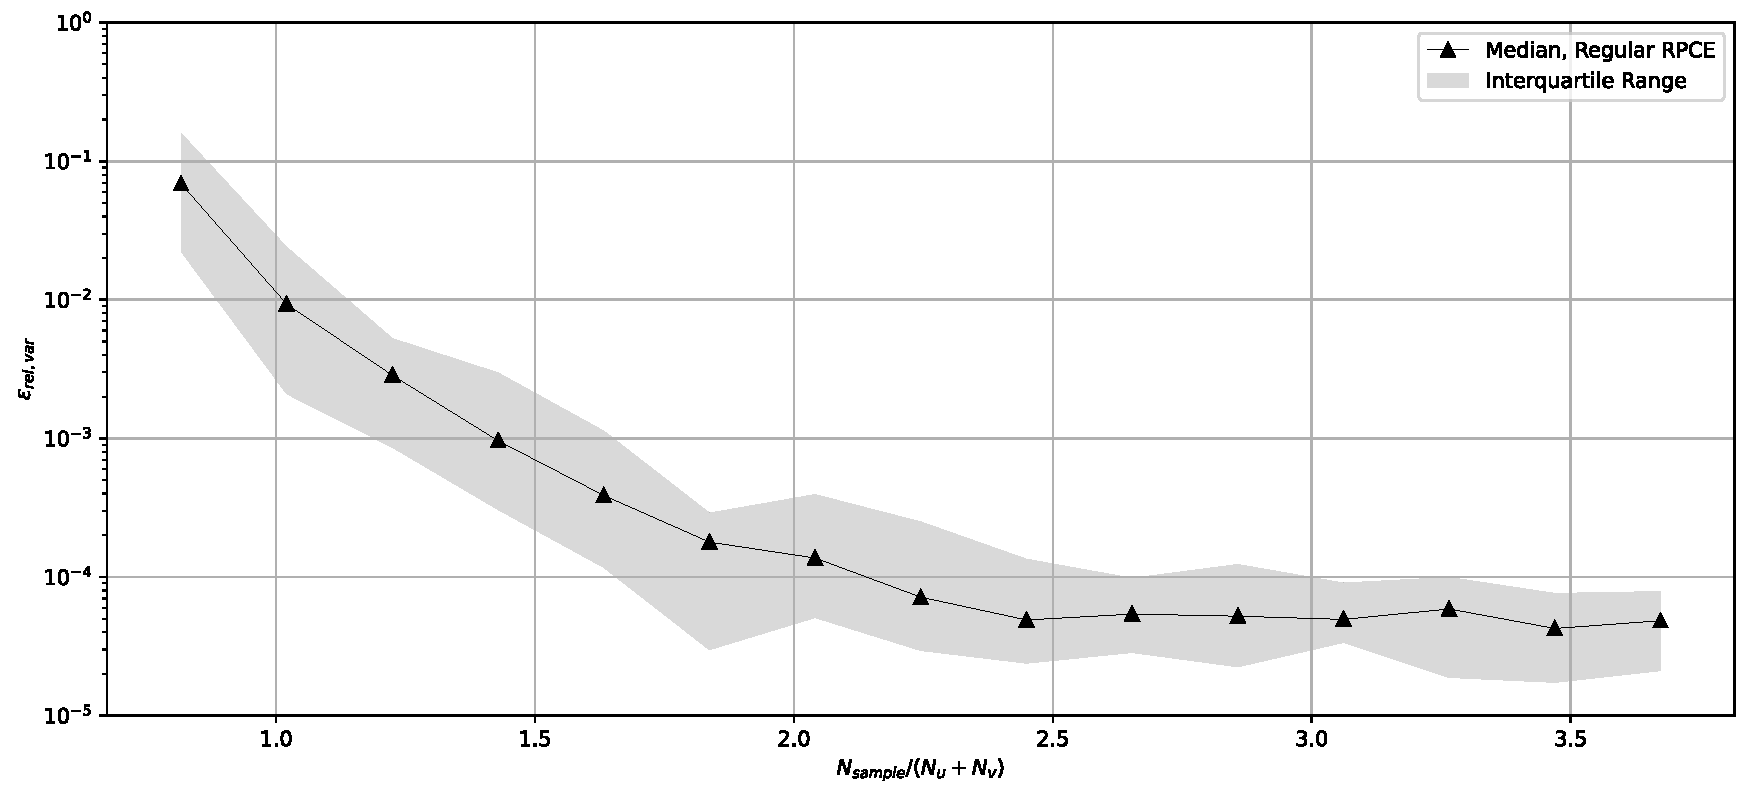
\includegraphics[width=1.0\textwidth]{
        plots/surrogate/plot_3P_B_16.pdf
    }
    \caption{%
        Relative Variance Errors of $H_{BA}$ for Regular RPCE Models at $\omega=16.0$ rad/s
    }
    \label{var_rRPCE_B_A_16}
\end{figure}
Similar to the relative empirical errors, the medians of the relative mean errors and relative variance errors converge when the size of training data is approximately $2.0$ to $2.5$ times the total number of bases in the models.

Subsequently, the author compares the relative errors for regular and sparse RPCE models.
Figures \ref{mean_sRPCE_B_A_16} and \ref{var_sRPCE_B_A_16} show the relative mean errors and relative variance errors of the FRF approximations for regular and sparse RPCE models at $\omega=16.0$ rad/s.
\begin{figure}[H]
    \centering
    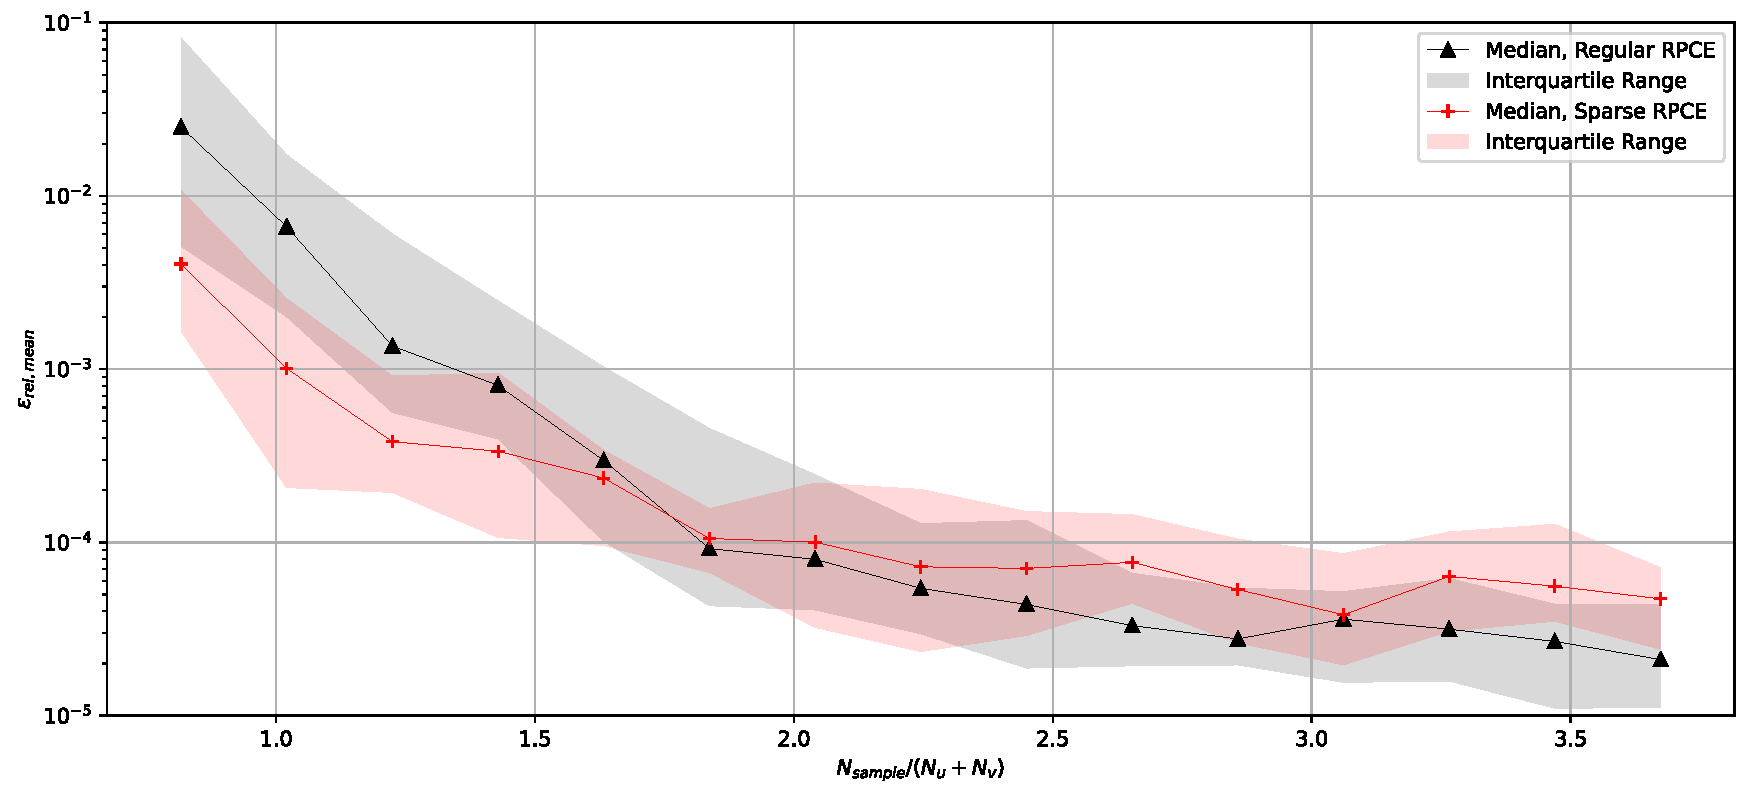
\includegraphics[width=1.0\textwidth]{
        plots/surrogate/plot_2_B_16.pdf
    }
    \caption{%
        Relative Mean Errors of $\left|H_{BA}\right|$ for Regular and Sparse RPCE Models at $\omega=16.0$ rad/s
    }
    \label{mean_sRPCE_B_A_16}
\end{figure}
\begin{figure}[H]
    \centering
    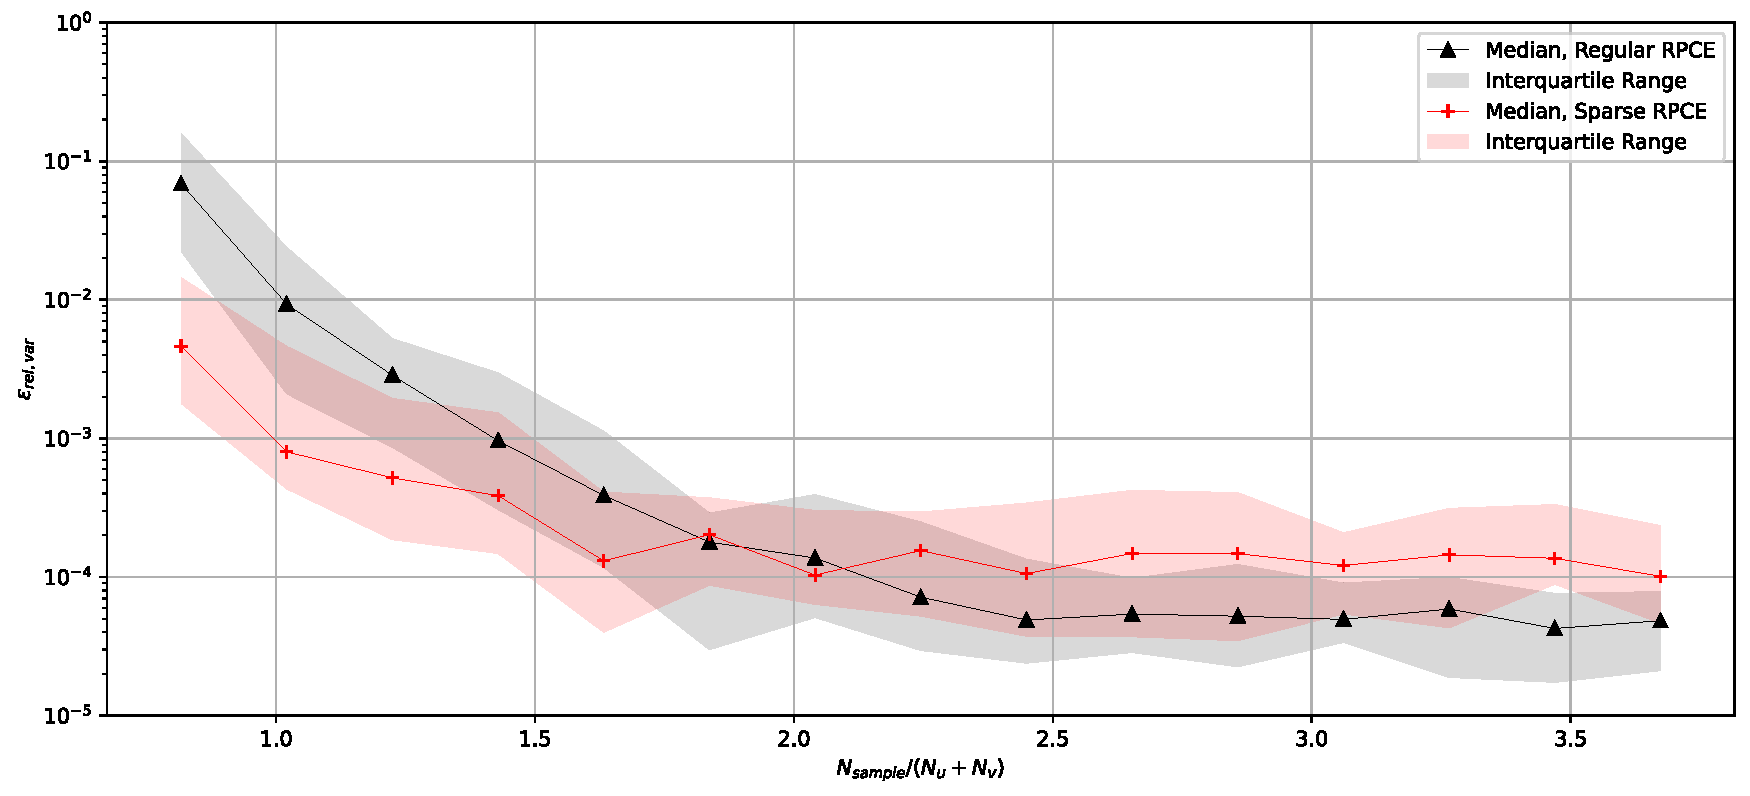
\includegraphics[width=1.0\textwidth]{
        plots/surrogate/plot_3_B_16.pdf
    }
    \caption{%
        Relative Variance Errors of $H_{BA}$ for Regular and Sparse RPCE Models at $\omega=16.0$ rad/s
    }
    \label{var_sRPCE_B_A_16}
\end{figure}
The two figures above show that the sparse RPCE models have lower relative mean errors and relative variance errors when training data sizes are small.
Figures \ref{mean_sRPCE_B_A_17} to \ref{mean_sRPCE_B_A_19} display the relative mean errors of the FRF approximations for regular and sparse RPCE models at various frequencies.
Figures \ref{var_sRPCE_B_A_17} to \ref{var_sRPCE_B_A_19} display the relative variance errors of the FRF approximations for regular and sparse RPCE models at various frequencies.
All figures show similar trends.
% The relative mean errors and relative variance errors at other frequencies are available in the appendix.
\begin{figure}[H]
    \centering
    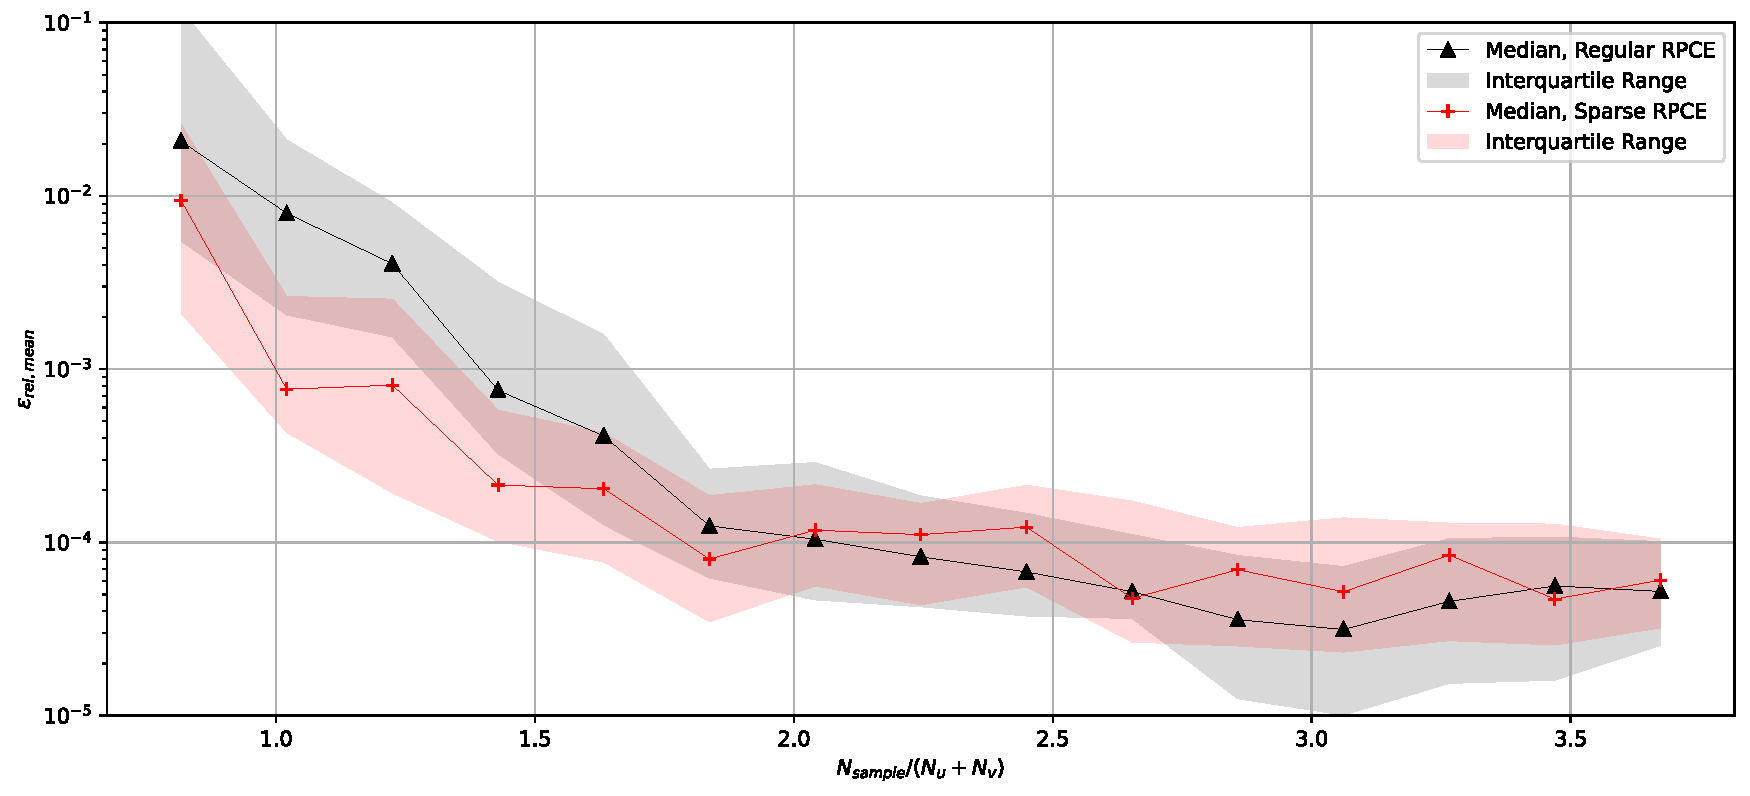
\includegraphics[width=1.0\textwidth]{
        plots/surrogate/plot_2_B_17.pdf
    }
    \caption{%
        Relative Mean Errors of $\left|H_{BA}\right|$ for Regular and Sparse RPCE Models at $\omega=16.5$ rad/s
    }
    \label{mean_sRPCE_B_A_17}
\end{figure}
\begin{figure}[H]
    \centering
    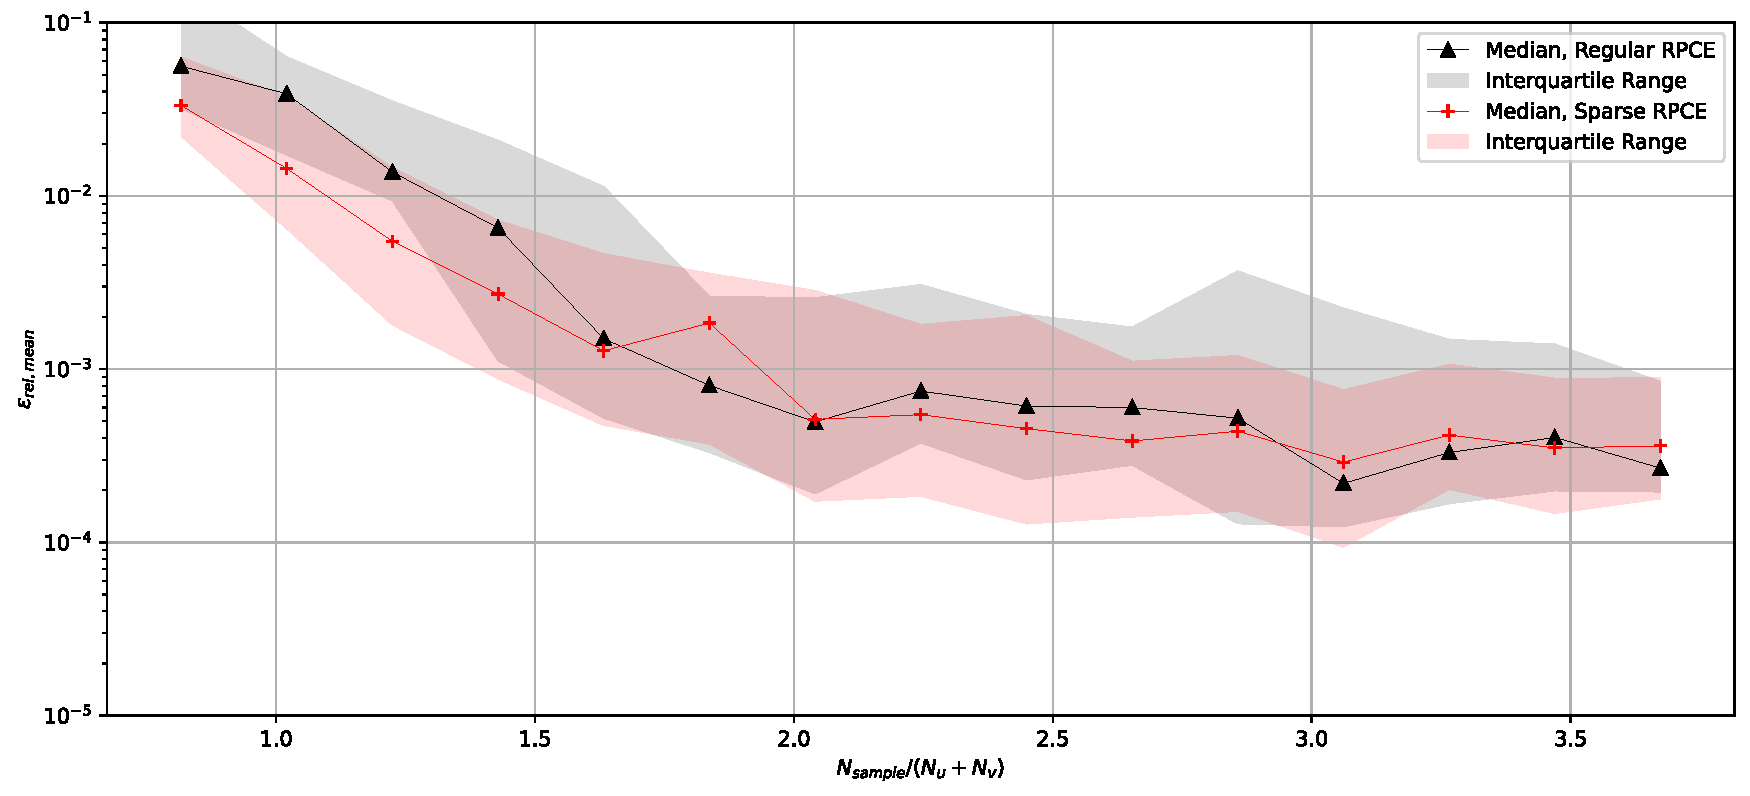
\includegraphics[width=0.85\textwidth]{
        plots/surrogate/plot_2_B_18.pdf
    }
    \caption{%
        Relative Mean Errors of $\left|H_{BA}\right|$ for Regular and Sparse RPCE Models at $\omega=17.0$ rad/s
    }
\end{figure}
\begin{figure}[H]
    \centering
    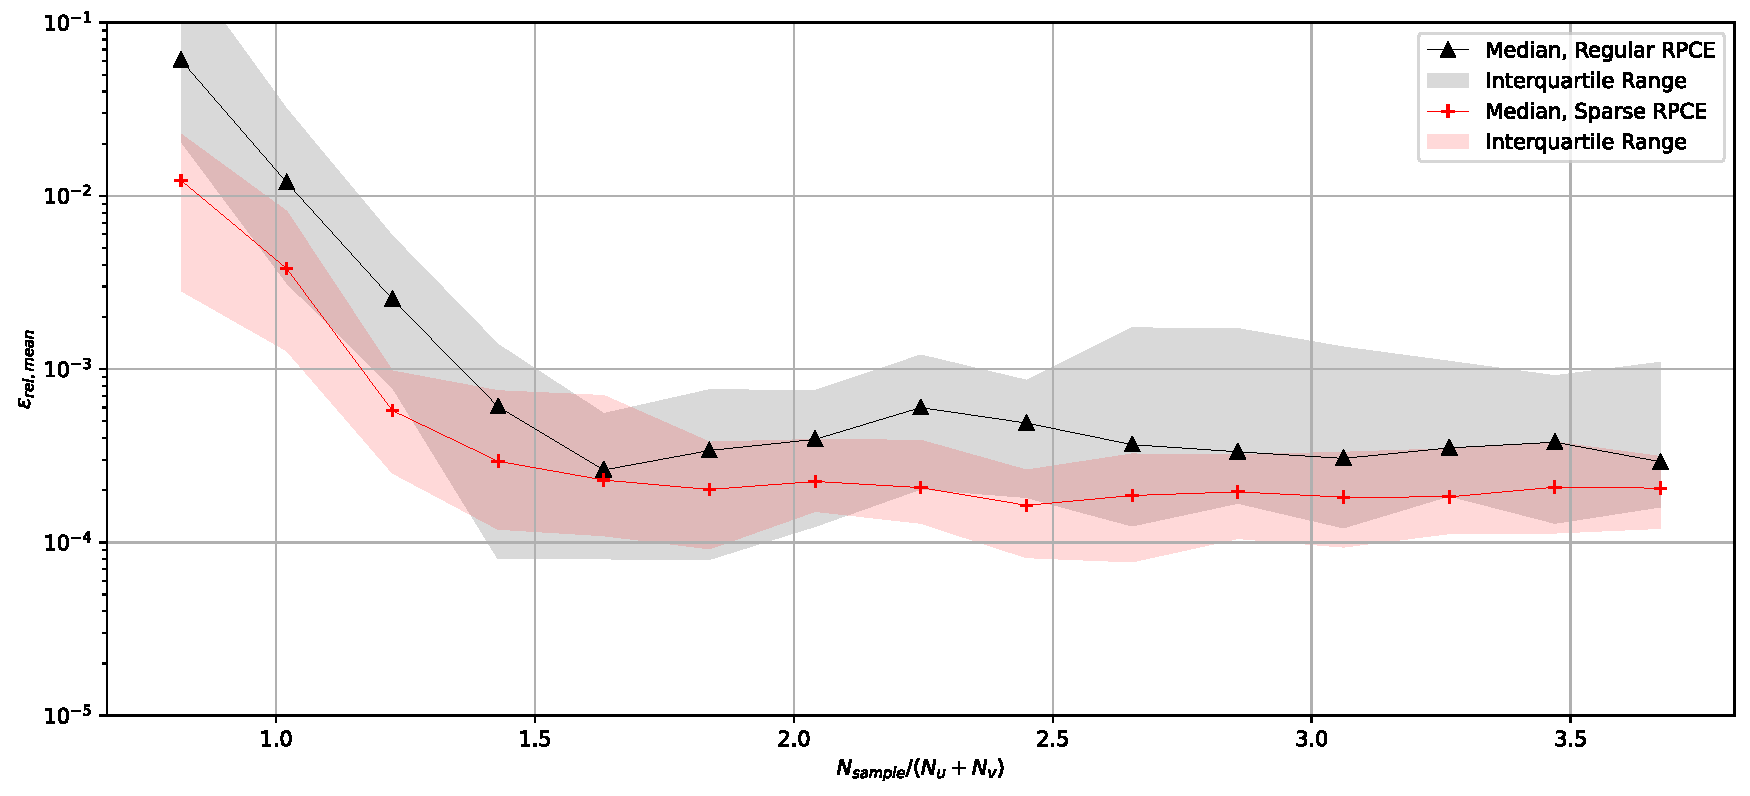
\includegraphics[width=0.85\textwidth]{
        plots/surrogate/plot_2_B_19.pdf
    }
    \caption{%
        Relative Mean Errors of $\left|H_{BA}\right|$ for Regular and Sparse RPCE Models at $\omega=17.5$ rad/s
    }
    \label{mean_sRPCE_B_A_19}
\end{figure}
\begin{figure}[H]
    \centering
    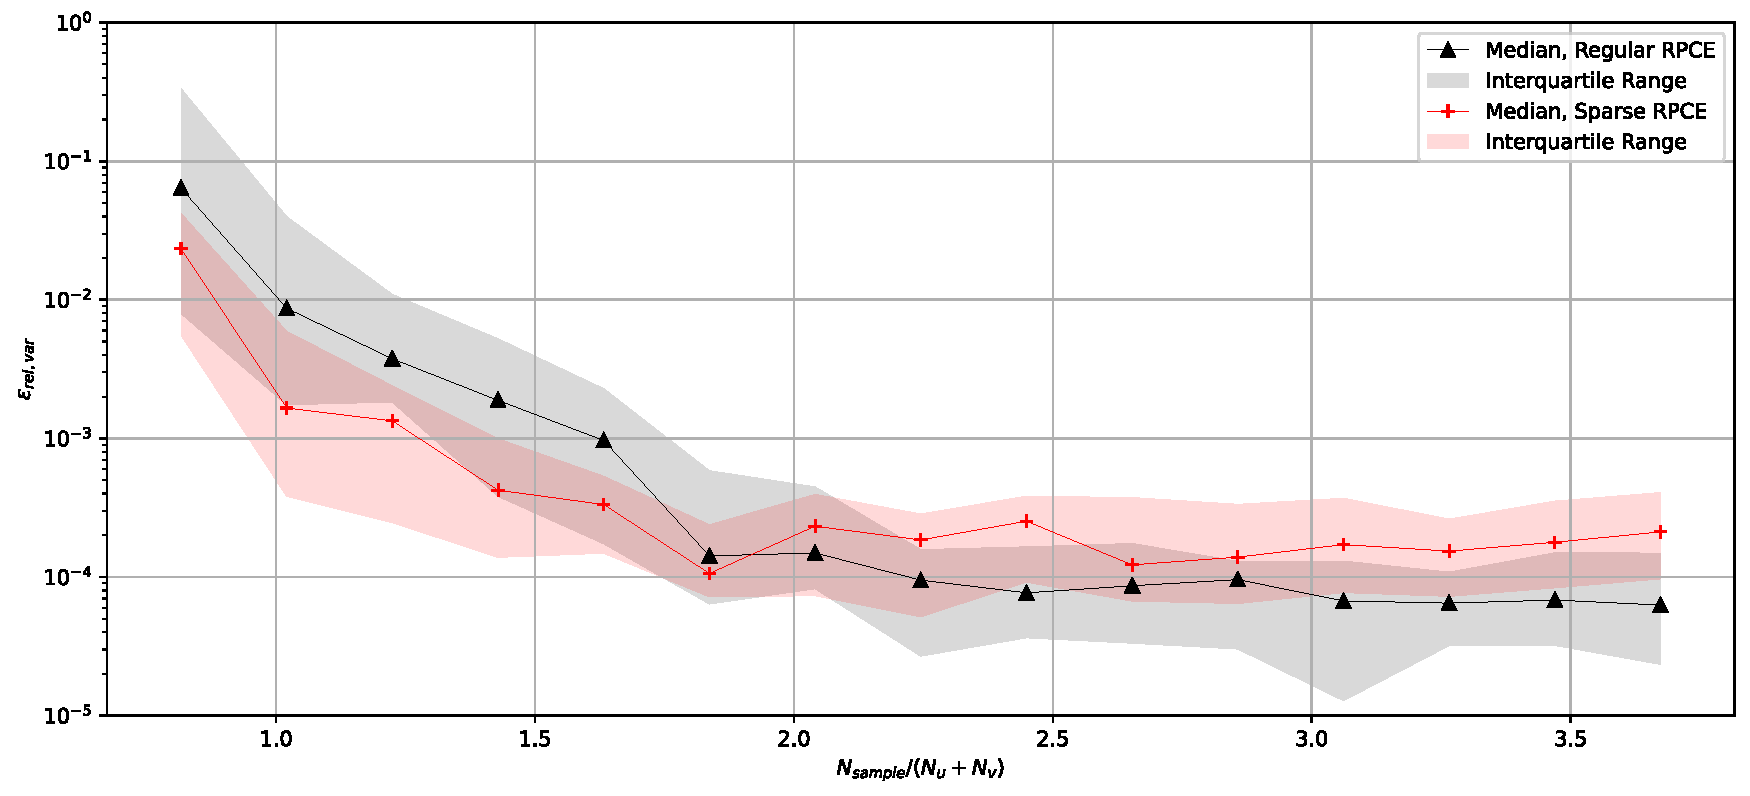
\includegraphics[width=0.85\textwidth]{
        plots/surrogate/plot_3_B_17.pdf
    }
    \caption{%
        Relative Variance Errors of $H_{BA}$ for Regular and Sparse RPCE Models at $\omega=16.5$ rad/s
    }
    \label{var_sRPCE_B_A_17}
\end{figure}
\begin{figure}[H]
    \centering
    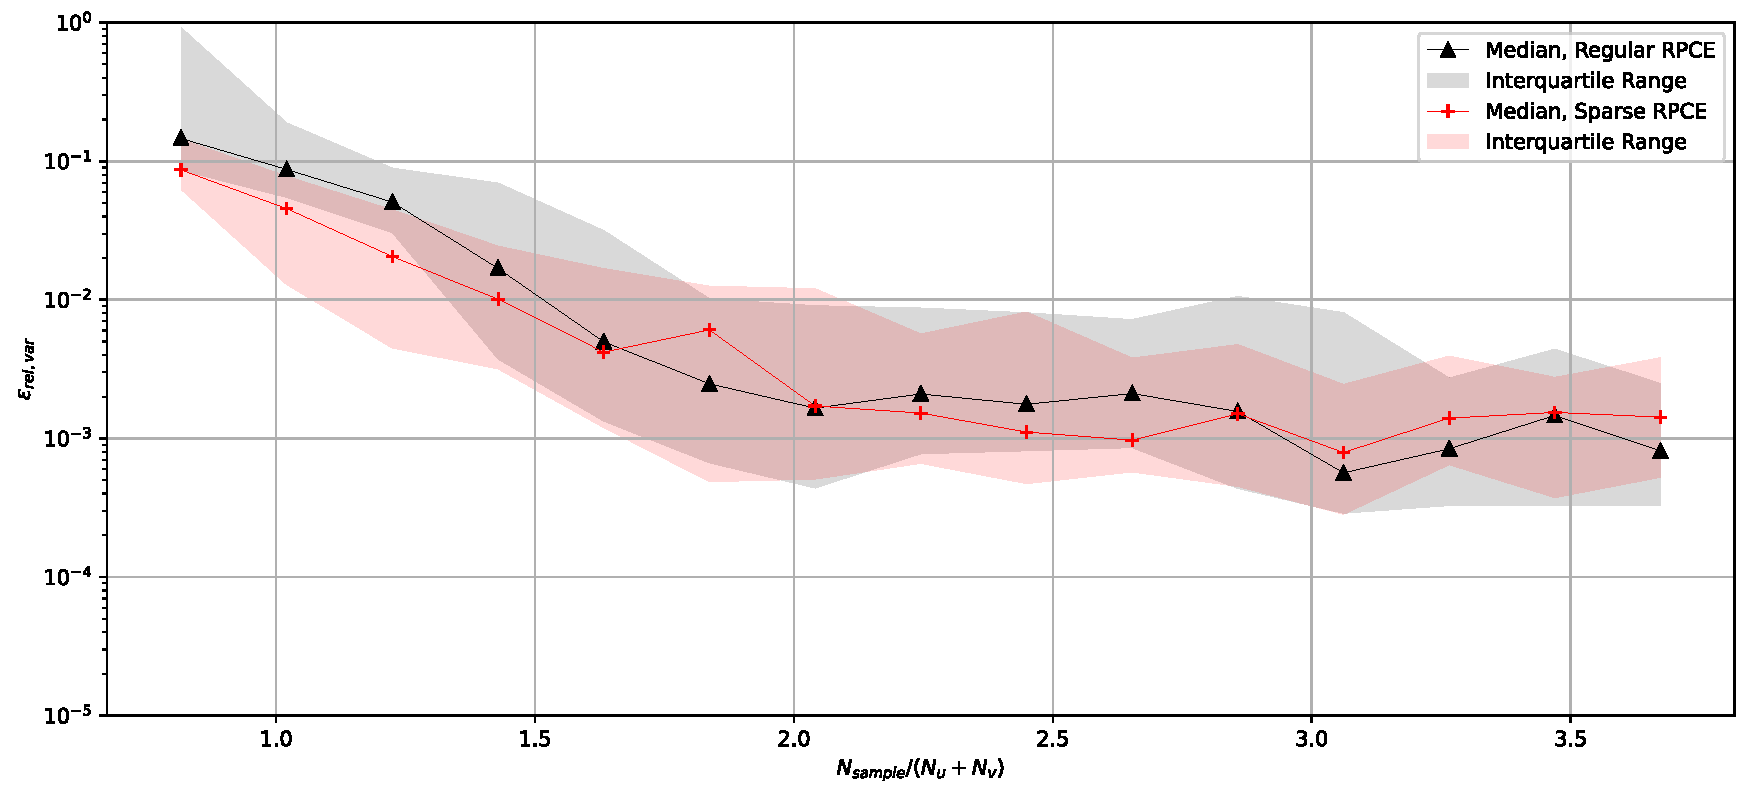
\includegraphics[width=0.85\textwidth]{
        plots/surrogate/plot_3_B_18.pdf
    }
    \caption{%
        Relative Variance Errors of $H_{BA}$ for Regular and Sparse RPCE Models at $\omega=17.0$ rad/s
    }
\end{figure}
\begin{figure}[H]
    \centering
    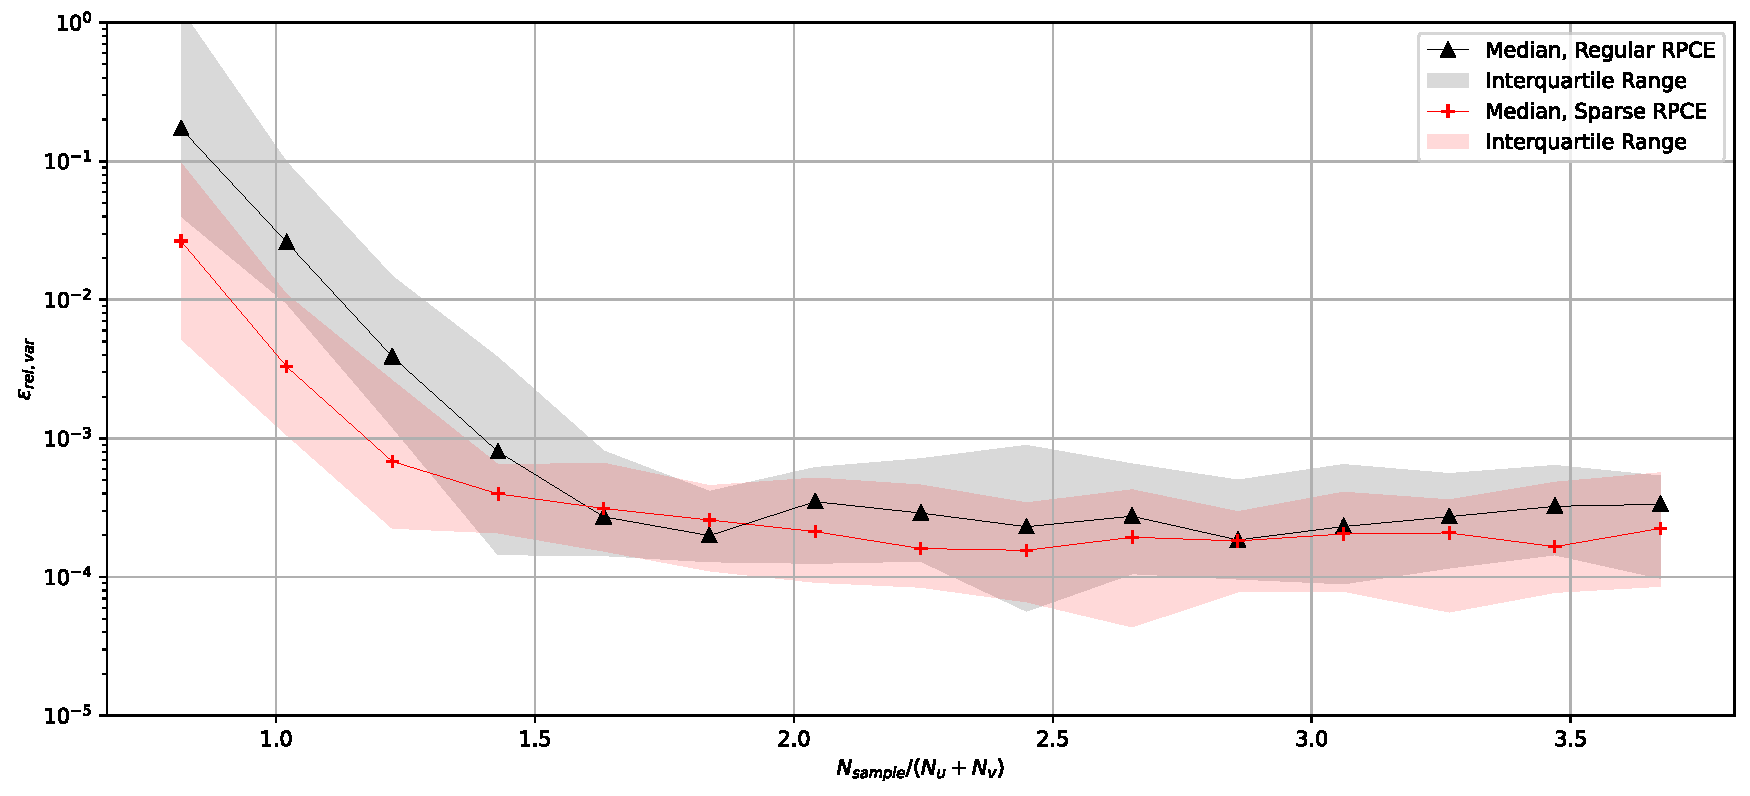
\includegraphics[width=0.85\textwidth]{
        plots/surrogate/plot_3_B_19.pdf
    }
    \caption{%
        Relative Variance Errors of $H_{BA}$ for Regular and Sparse RPCE Models at $\omega=17.5$ rad/s
    }
    \label{var_sRPCE_B_A_19}
\end{figure}